\documentclass[border=8pt]{standalone}
\usepackage{xcolor}
\definecolor{deepblue}{RGB}{31,84,150}
\definecolor{steel}{RGB}{70,130,180}
\definecolor{crimsonred}{RGB}{190,30,60}
\definecolor{darkorang}{RGB}{230,140,20}
\definecolor{seagreen}{RGB}{0,128,60}
\usepackage{pgfplots}
\pgfplotsset{compat=1.18}
\begin{document}
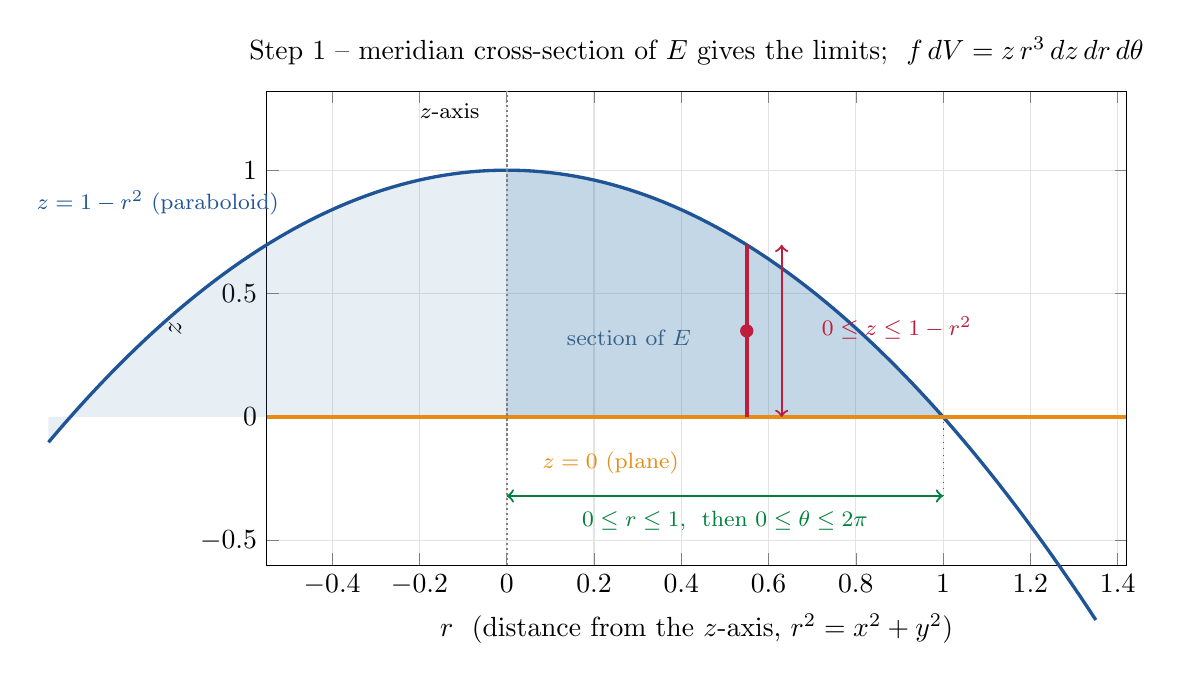
\begin{tikzpicture}
\begin{axis}[
    width=12.5cm, height=7.6cm,
    xmin=-0.55, xmax=1.42, ymin=-0.60, ymax=1.32,
    xlabel={$r$ \ (distance from the $z$-axis, $r^2=x^2+y^2$)},
    ylabel={$z$},
    grid=major, grid style={gray!22},
    title={Step 1 -- meridian cross-section of $E$ gives the limits; \ $f\,dV=z\,r^{3}\,dz\,dr\,d\theta$},
    every title/.append style={font=\small},
    clip=false,
]
% --- mirrored half of the section (light) -----------------------------------
\addplot[fill=steel, opacity=0.13, draw=none, domain=-1.05:0, samples=80] {1-x^2} \closedcycle;
% --- shaded region 0 <= r <= 1, 0 <= z <= 1 - r^2 ---------------------------
\addplot[fill=steel, opacity=0.32, draw=none, domain=0:1, samples=80] {1-x^2} \closedcycle;
% --- paraboloid profile ------------------------------------------------------
\addplot[deepblue, very thick, domain=-1.05:1.35, samples=120] {1-x^2};
% --- plane z = 0 -------------------------------------------------------------
\addplot[darkorang, very thick, domain=-0.55:1.42, samples=2] {0};
% --- direct labels -----------------------------------------------------------
\node[deepblue, font=\footnotesize, anchor=south east] at (-0.50,0.78)
    {$z=1-r^2$  (paraboloid)};
\node[darkorang, font=\footnotesize, anchor=north west] at (0.06,-0.10)
    {$z=0$  (plane)};
\node[steel!75!black, font=\footnotesize, align=center] at (0.28,0.32)
    {section of $E$};
% --- z-axis ------------------------------------------------------------------
\draw[gray, thick, densely dotted] (0,-0.60) -- (0,1.32);
\node[font=\footnotesize, anchor=east] at (-0.04,1.24) {$z$-axis};
% --- vertical element at r0 = 0.55 ------------------------------------------
\draw[crimsonred, ultra thick] (0.55,0) -- (0.55,0.6975);
\fill[crimsonred] (0.55,0.3488) circle (2.4pt);
\draw[<->, crimsonred, thick] (0.63,0) -- (0.63,0.6975);
\node[crimsonred, font=\footnotesize, align=left, anchor=west] at (0.70,0.36)
    {$0\le z\le 1-r^2$};
% --- r-range arrow -----------------------------------------------------------
\draw[<->, seagreen, thick] (0,-0.32) -- (1,-0.32);
\draw[seagreen, dotted, thin] (1,-0.32) -- (1,0);
\node[seagreen, font=\footnotesize, anchor=north] at (0.5,-0.34)
    {$0\le r\le 1$, \ then $0\le\theta\le 2\pi$};
\end{axis}
\end{tikzpicture}
\end{document}
